The Johnson-Lindenstrauss and MinHash methods have been implemented (see~\hyperref[ch:appendix]{Appendix}) and tested on a set of \( 1000 \) compounds randomly selected from the original datasets using the bash terminal \texttt{shuf} command. The parameters used for the analysis were \( r = 3 \) and \( N \in \set{128, 512, 2048} \), so \( N \sim \log(m)\epsilon^{-2} \) for \( m = 1000 \) and \( 0.05 \leq \epsilon \leq 0.25 \).

The goal of the experiment was to compare the approaches to dimensionality reduction of~the encodings, by evaluating how well each method preserved the pairwise similarity between the compounds. The Johnson-Lindenstrauss and MinHash methods were compared to manipulating the length of the fingerprints modulo the value of \( N \). The \autoref{fig:reduced} shows how the distribution of distances in the Jaccard metric has changed for the studied methods.
\begin{figure}[H]
    \centering
    a) The random dataset
    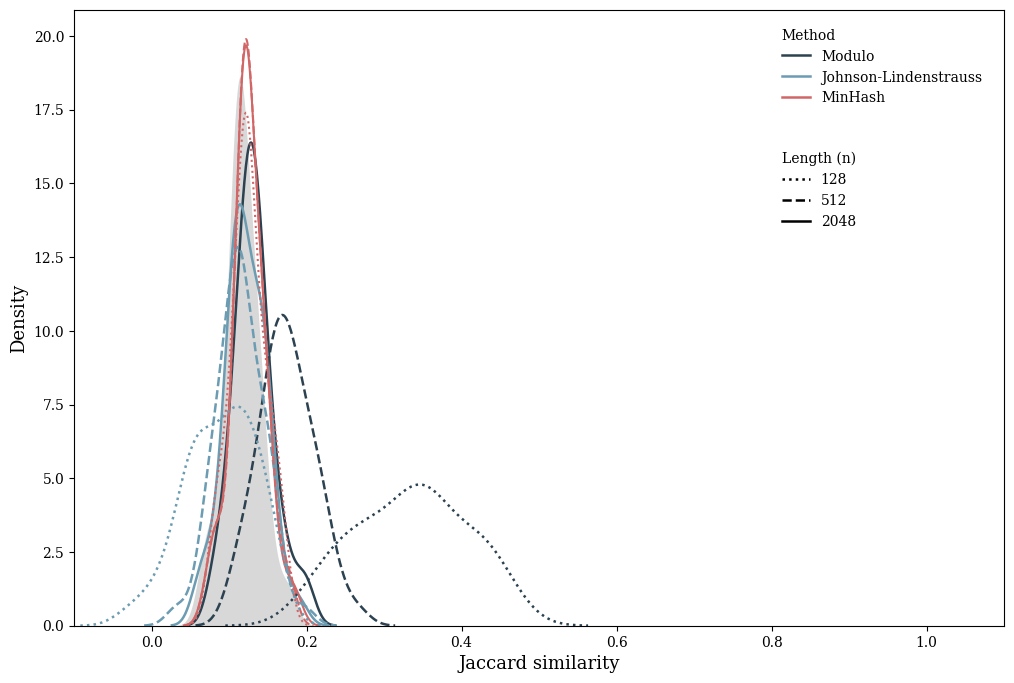
\includegraphics[width=0.8\textwidth]{figures/reduced.png}
\end{figure}
\begin{figure}[H]
    \centering
    b) The hydrocarbon dataset
    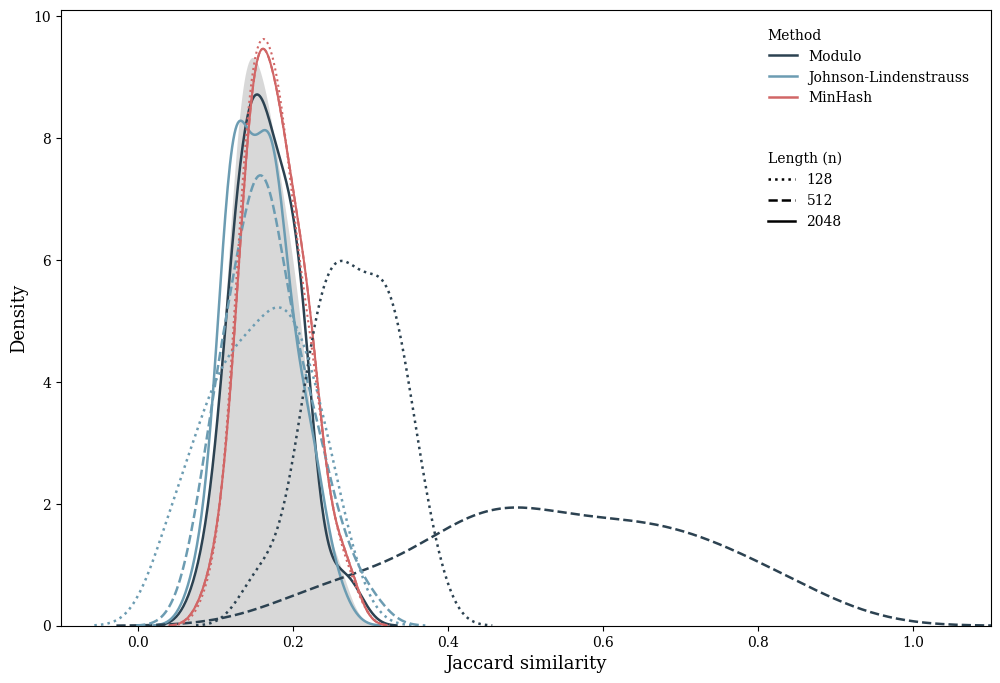
\includegraphics[width=0.8\textwidth]{figures/reduced_c22.png}
    \caption{Distribution of distance in Jaccard metric for the encodings reduced with different methods}
    \label{fig:reduced}
\end{figure}
For the original non-reduced fingerprints from the random dataset, Jaccard distance ranged from \( 0.871 \) to \( 0.985 \) with a mean of \( 0.933 \). For \( N = 8192 \), the distributions of distances for reduced encodings did not differ much from the original distributions. For smaller values of \( N \), however, the Johnson-Lindenstrauss and MinHash methods outperformed the naive method. Reducing the fingerprint length modulo \( N \) lead to visibly broadened distribution. For \( N = 128 \), the mean distance was equal to \( 0.715 \) with the most similar pair of compounds having distance of \( 0.587 \). For both other methods, the absolute difference in pairwise distance compared to the original one in no case exceeded \( 0.10 \) for the Johnson-Lindenstrauss and \( 0.03 \) for the MinHash reduction.